\documentclass[a4paper,openright,12pt]{article}
\usepackage[utf8]{inputenc}
\usepackage{graphicx} 
\usepackage{subfigure}
\usepackage{caption}
\usepackage{subcaption}
\usepackage[mathscr]{eucal}
\usepackage{titling}
\usepackage{float}
\usepackage{amsmath}
\usepackage{afterpage}
\usepackage{vmargin}
\usepackage[spanish]{babel}
\usepackage{eurosym} 
\usepackage{multirow} 
\usepackage{cite}
\usepackage{url}

\setpapersize{A4}   %  DIN A4
\setmargins{3cm}    % margen izquierdo
{3.5cm}             % margen superior
{15cm}              % anchura del texto
{22.5cm}            % altura del texto
{10pt}              % altura de los encabezados
{1cm}               % espacio entre el texto y los encabezados
{0pt}               % altura del pie de página
{2cm}               % espacio entre el texto y el pie de página

\begin{document}

\begin{titlepage}
    \begin{center}
        \vspace*{-1in}
        \begin{figure}[htb]
            \begin{center}
                
\includegraphics[width=8cm]{udc.eps}
            \end{center}
        \end{figure}

        \vspace*{1in}
        PROGRAMACIÓN DE SISTEMAS 22/23 Q1\\
        \begin{figure}[htb]
            \begin{center}
                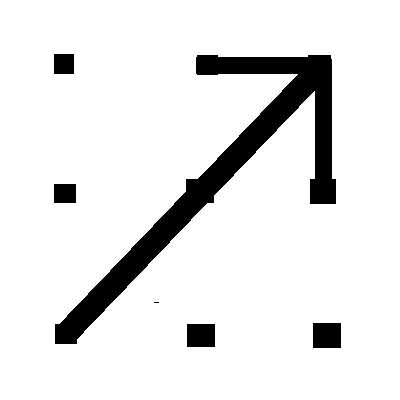
\includegraphics{icon.png}
            \end{center}
        \end{figure}
        \vspace*{1in}
        \begin{Large}
            \textbf{MallaVectores} \\
        \end{Large}
        
        \vspace*{3in}
        
        \begin{large}
            \raggedleft
            \textbf{Autores:}Iago Valeiro Castrillón \\
            Alejandro Dopazo López \\
            Alberto Ferreiro Campello \\
            \textbf{Fecha:}\textit{A Coruña, 17 Octubre 2022}\\
        \end{large}
        
    \end{center}
\end{titlepage} 

\newpage

\addtocontents{toc}{\hspace{-7.5mm} \textbf{Capítulos}}
\addtocontents{toc}{\hfill \textbf{Página} \par}
\addtocontents{toc}{\vspace{-2mm} \hspace{-7.5mm} \hrule \par}

\pagenumbering{empty}

\tableofcontents

\vspace{5cm}

\begin{flushright}
    \begin{table}[hbtp]
        \begin{center}
        
            \caption{Tabla de versiones.}
            \label{tabla:versiones}
            \small
            \vspace{1ex}
            
            \begin{tabular}{|c|c|l|}
                \hline
                Versión & Fecha & Autor \\
                \hline \hline
                x & y & \\ \hline
                x & y & \\ \hline
                x & y & \\ \hline
            \end{tabular}
            
        \end{center}
    \end{table}
\end{flushright}

\newpage
\pagenumbering{arabic}


%%%%%%%
%%%%%%%
\section{Introducción}\label{cap.introduccion}
La aplicación propuesta consiste en un editor de imágenes vectoriales para dispositivos móviles Android, inicialmente sería para la creación de iconos y basaría su funcionamiento en la interconexión de puntos en una malla cuadriculada, además llevaría integrado un sistema de control de versiones basado en git que además de permitir guardar un historial de cambios, añadiría la funcionalidad de almacenamiento en la nube para las imágenes exportadas.

%%
\subsection{Objetivos}
\begin{enumerate}
    \item Principal:
    \begin{itemize}
        \item Creación de imágenes vectoriales a partir de puntos, líneas y curvas.
    \end{itemize}

    \item Secundarios:
    \begin{itemize}
        \item Exportación de las imágenes a formatos de archivo habituales como \\
        .svg~\cite{SVG} que permitan compartirlas con otros usuarios.
        \item Manejo de los cambios en las imágenes mediante un sistema de control de versiones integrado como puede ser el proporcionado por Git a través de la librería JGit~\cite{JGit}.
    \end{itemize}
\end{enumerate}

Las dependencias son las especificadas en la sección \emph{Funcionalidades}

%%
\subsection{Motivación}
Crear una herramienta con la que poder experimentar fácil y cómodamente con gráficos vectoriales, se trata de un tema de especial interés dada la relativa carencia de herramientas destinadas a estos fines.
Es aplicable para, por ejemplo, el diseño de recursos para aplicaciones gráficas, principalmente iconos.

%%
\subsection{Trabajo relacionado}
\begin{itemize}
    \item Dot Matrix~\cite{Dot_Matrix}, se trata de la aplicación original que dio pié a este proyecto, consta de un editor de iconos desarrollado para Linux por un equipo de 10 personas en el lenguaje de programación Vala~\cite{Vala}. Se puede ver en la figura \ref{fig:trabajo_relacionado}.\subref{fig:dot_matrix}.
    \item Gráficos Vectoriales~\cite{Graficos_Vectoriales} en este caso se trata de una aplicación Android similar a la que se plantea, es bastante completa y se oferta como conversor de archivos .png y .jpg a .svg. Se puede ver en la figura \ref{fig:trabajo_relacionado}.\subref{fig:graficos_vectoriales_app}.
\end{itemize}

\begin{figure}
    \hfill
    \subfigure[Dot Matrix\label{fig:dot_matrix}]{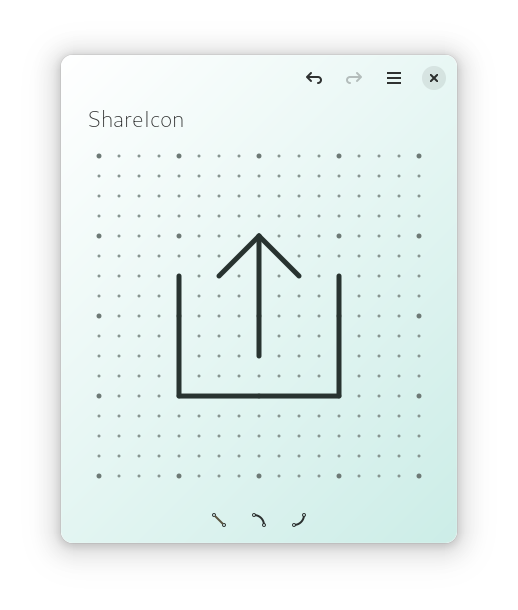
\includegraphics[width=7.5cm]{imagenes/dot_matrix_original.png}}
    \hfill
    \subfigure[Graficos Vectoriales\label{fig:graficos_vectoriales_app}]{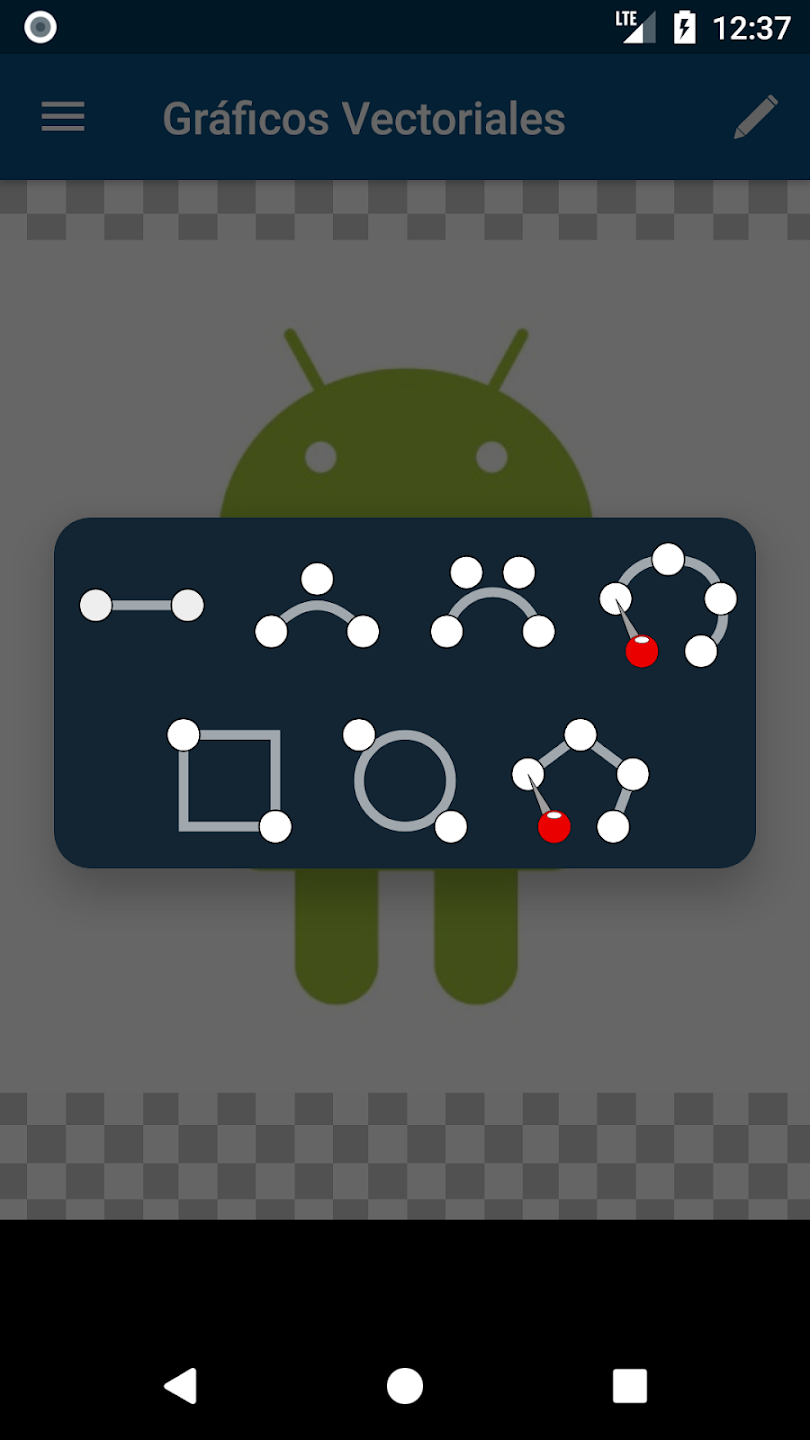
\includegraphics[width=7cm]{imagenes/graficos_vectoriales_app.png}}
    \hfill
    \caption{Ejemplos de aplicaciones similares.}
    \label{fig:trabajo_relacionado}
\end{figure}

%%%%%%%
%%%%%%%
\section{Análisis de requisitos}
\begin{itemize}
    \item La aplicación debe ser capaz de permitir al usuario realizar dibujos utilizando gráficos vectoriales que permitan ser redimensionados sin perder calidad.
    \item Dichos dibujos pueden incuír líneas rectas y curvas, la aplicación que se desarrolle debe dar soporte a ambas.
    \item Con el objetivo de facilitar el proceso de dibujado, si dos vértices están muy próximos estos deberían unirse de forma automática. Dicho de otro modo, los puntos de inicio y fin de cada línea deben ser fijos, dispuestos en una cuadrícula de puntos.
    \item Se espera que la aplicación incluya una opción habitual de los editores de imágenes como es "deshacer".
    \item La aplicación debe permitir exportar los dibujos a formatos de archivo habituales.
    \item Dichos archivos deben poderse compartir.
\end{itemize}

%%
\subsection{Funcionalidades}
\subsubsection{Creación de imágenes vectoriales}
Se pueden disponer los siguientes elementos en la pantalla:
\begin{itemize}
	\item Líneas rectas.
	\item Curvas de Bézier~\cite{Curvas_de_Bezier} cúbicas.
	\item Curvas de Bézier cuadráticas.
\end{itemize}

Cada tipo de elemento tiene un modo asociado,
que se puede seleccionar mediante
la barra de botones de la actividad principal.
Los modos están identificados por las letras  'L', 'Q' y 'C' para
las líneas rectas y las curvas cuadráticas y cúbicas, respectivamente.

El modo actual se muestra al principio de la barra de botones.

Las líneas rectas se dibujan arrastrando entre los dos puntos que
vayan a definirla.

Las curvas se definen pulsando primero en cada punto de la recta 
y luego en sus puntos de control.
Las curvas cuadráticas tienen un punto de control y las cúbicas dos.

\subsubsection{Exportación a ficheros}
Depende de la funcionalidad \emph{Creación de imágenes vectoriales}.
Las imágenes generadas se pueden exportar a ficheros externos en formato svg. El formato usado se ceñirá a la especificación SVGTiny~\cite{SVGTiny} excepto las funciones de text, al igual que los VectorDrawable de android~\cite{VectorDrawable}.

%%

\subsection{Integración con control de versiones}
Se podrán integrar los proyectos con el sistema de control de versiones Git~\cite{Git}. Se podrán realizar las siguientes acciones:
\begin{itemize}
    \item Revisar el registro de commits.
    \item Realizar commits.
    \item Crear ramas.
    \item Ver las ramas disponibles.
    \item Fusionar ramas.
\end{itemize}

%%

\subsection{Guardado automático de los ficheros}
Habrá un servicio en segundo plano que guarde las imágenes creadas a un fichero de forma automática cada cierto tiempo, el cual será ajustable mediante la propia aplicación. Ésto se podrá desactivar completamente mediante la propia aplicación.

%%
\subsection{Prioridades}
La funcionalidad \emph{Exportación a ficheros} depende de la funcionalidad \emph{Creación de imágenes vectoriales}.
La funcionalidad \emph{Integración con control de versiones} depende de la funcionalidad \emph{Exportación a ficheros}.
La funcionalidad \emph{Guardado automático de los ficheros} depende de la funcionalidad \emph{Exportación a ficheros}.

\emph{Creación de imágenes vectoriales} tiene la mayor prioridad, seguida de \emph{Exportación a ficheros}, la cual es sucedida por \emph{Integración con control de versiones}.

%%%%%%%
%%%%%%%
\section{Planificación inicial}

%%
\subsection{Iteraciones}\label{iteraciones}
Primera iteración: Implementación de la funcionalidad \emph{Exportación a ficheros} y \emph{Creación de imágenes vectoriales}.

Segunda iteración: Implementación de la funcionalidad \emph{Exportación a ficheros}.

Tercera iteración: Implementación de la funcionalidad \emph{Integración con control de versiones}.

Cuarta iteración: Implementación de la funcionalidad \emph{Guardado automático de los ficheros}.

Posiblemente otras iteraciones, dependiendo del curso del desarrollo: Expansión de funcionalidades; por ejemplo, posibilitar la interacción con otros elementos del estándar SVGTiny~\cite{SVGTiny}, como rellenos y colores, o posibilitar la exportación a distintos formatos.


%%
\subsection{Responsabilidades}
Iago Valeiro Castrillón: 
\emph{Creación de imágenes vectoriales}, 
\emph{Guardado automático de los ficheros} e 
\emph{Integración con control de versiones}.

Alejandro Dopazo López:
\emph{Creación de imágenes vectoriales} e
\emph{Integración con control de versiones}

Alberto Ferreiro Campello:
\emph{Exportación a ficheros}, 
\emph{Guardado automático de los ficheros} e
\emph{Integración con control de versiones}.


%%
\subsection{Hitos}
Primer entregable: primera iteración implementada. Pruebas de las funcionalidades implementadas.

Segundo entregable: segunda iteración implementada. Pruebas de las funcionalidades implementadas.

Tercer entregable: tercera iteración implementada. Pruebas de las funcionalidades implementadas.

Entregable final: Pruebas de integración y de usabilidad. Revisión de las iteraciones anteriores.

%%
\subsection{Incidencias}
\begin{itemize}
    \item El proyecto transcurre demasiado rápido/despacio:
\end{itemize}
Se añadirán o quitarán iteraciones al proyecto de acuerdo a lo especificado en la sección \ref{iteraciones}. Los hitos y los entregables se ajustarán apropiadamente.

%%


%%%%%%%
%%%%%%%
\section{Diseño}
%%
\subsection{Arquitectura}

\subsubsection{Actividad principal}
MainActivity, con una barra con botones para seleccionar los modos de dibujo una Vistamalla que muestre la imagen en sí y responda a las acciones y un menú de opciones.

Desde del menú de opciones se puede:
\begin{itemize}
	\item exportar la imagen actual a un fichero.
    \item seleccionar un fichero o un repositorio git a abrir con un Intent implícito.
    \item Lanzar la actividad ControlVersiones.
    \item Lanzar la actividad Ajustes.
\end{itemize}
%%

\subsubsection{Vistamalla}
La vista muestra la malla de puntos y las formas dibujadas por el usuario.

También gestiona su propia interacción con el usuario.

\subsubsection{Actividad ControlVersiones}
Si hay un repositorio de git, se muestra una RecyclerView con un registro de commits.

Para operar con los repositorios, se usará la librería JGit\cite{JGit}.

Si no, se ofrece la opción de crear un repositorio de git con la imagen actual en una carpeta seleccionada con un intent implícito.

La actividad tiene botones para lanzar la actividad GestionRamas y el fragmento RealizarCommit, que muestra si se realizaron cambios y una entrada de texto para el mensaje del commit.
%%

\subsubsection{Actividad Ajustes}
Muestra una entrada para cambiar la frecuencia con la que se guarda automáticamente la imagen actual y un botón para deshabilitar el servicio GuardadoAutomatico.

%%

\subsubsection{Actividad GestionRamas}
Se muestran las ramas actuales con una ListView. Hay un FloatingActionButton para añadir ramas. Pulsar en una rama hace que se cambie a ella. Si se desliza una rama a la izquierda, se fusiona a la rama actual.
%%

\subsection{Persistencia}
Se almacenarán las imágenes y los repositorios en el sistema de ficheros.
También se almacenarán los ajustes del servicio de guardado automático.

\subsection{Vista}
Una actividad principal mostrando un menú con las acciones que se pueden realizar sobre la imagen actual, ordenados por la recencia de su uso. La actividad contiene el fragmento con la malla de puntos.

Desde el menú de la actividad principlal se puede navegar a las actividades de la gestión de versiones y de los ajustes.

La actividad del control de versiones muestra el registro de commits y la opción para añadir un commit. Desde ésta actividad se puede navegar a la de la gestión de las ramas.

En la actividad de la gestión de las ramas se muestran las ramas actuales y las opciones para añadir nuevas ramas y cambiar de ramas.

En la actividad de ajustes se muestra una entrada para cambiar la frecuencia con la que se guarda automáticamente la imagen actual y un botón para deshabilitar el servicio de guardado automático.

%%

\subsection{Comunicaciones}
Las imágenes y los proyectos de git se guardan en el sistema de ficheros local.
%%

\subsection{Sensores}
No se debería usar ninguno explícitamente aparte de la entrada por la pantalla táctil.
%%

\subsection{Background}
\subsubsection{Servicio GuardadoAutomatico}
Mientras el usuario va haciendo su diseño podrá ir guardando sus 
avances, aunque el sistema irá guardandolo de manera automática para
evitar que se pierda información por culpa de un cierre inesperado
de la aplicación.

El guardado sucederá mediante el servicio GuardadoAutomatico. Éste sucederá cada vez que pase un período definido en la actividad Ajustes.
%%

%%%%%%%
%%%%%%%

\bibliographystyle{pfc-fic}
\bibliography{biblio}
\addcontentsline{toc}{section}{Bibliografía}

\end{document}
